\FloatBarrier
\section{Archived experiments}\label{sec:archived}
The following results retain the original condition-specific sampling protocol. They are reported for transparency and historical comparison, not pooled with the document-paired validation. Sample sizes match across archived conditions but article identities generally differ. All numbers, figures and inferential summaries in this appendix refer to the archived protocol. Statements such as ``same samples'' in the model description mean shared across models for a given condition, not shared across conditions. The main results and conclusions use Section~\ref{sec:paired}. The exploratory source split, temporal masking and duplicate-removal check were not repeated with paired sampling.

\subsection{TF-IDF: pooled results}
Table~\ref{tab:pooled} and Fig.~\ref{fig:gap} give the pooled results. The baseline AUC gap is 0.213. Applying all three interventions gives 0.160, which removes 24.7\% of the gap (95\% interval 21.6--27.8\%; computed per seed and averaged, not from the rounded pooled gaps). The reduction comes from length matching and entity masking: L+E alone removes 27.3\% (24.8--29.7\%), slightly more than all three together, because source masking does not reduce the gap (its estimated contribution is $-2.3\%$ \ci{-4.9}{0.3}) and slightly lowers transfer. Random-deletion controls do not reduce the gap either: it stays at 0.212--0.223 against a baseline of 0.213, and $R_E$ and $R_{SE}$ lower cross-dataset AUC by about 0.006 and 0.011. The factorial effects on the AUC gap (Table~\ref{tab:effects}) are $-0.036$ for L and $-0.022$ for E, with interactions of at most 0.002 in magnitude, so the effects are close to additive. Length matching raises cross-dataset AUC from 0.772 to 0.806 while leaving in-domain AUC unchanged (0.985): the gap shrinks because transfer improves, not because in-domain performance falls.

Against matched random deletion, entity masking raises cross-dataset AUC by 0.020 \ci{0.016}{0.024} and changes the gap by $-0.025$ \ci{-0.028}{-0.022}. Source masking has the opposite effect: cross-dataset AUC changes by $-0.014$ \ci{-0.019}{-0.009} and the gap grows by 0.006 \ci{0.001}{0.011}. Both comparisons have the same sign in all eight seeds.

\begin{table}[t]
\caption{Archived protocol: TF-IDF + LR, pooled over the six ordered pairs, eight seeds. In-domain AUC, cross-dataset AUC and AUC gap with 95\% intervals over seeds.}
\label{tab:pooled}
\centering\footnotesize
\adjustbox{max width=\linewidth}{\begin{tabular}{@{}lccc@{}}
\toprule
Condition & In AUC & Cross AUC & Gap\\
\midrule
C0 (baseline) & 0.985 & 0.772 \ci{.770}{.775} & 0.213 \ci{.210}{.216}\\
S & 0.977 & 0.760 \ci{.755}{.764} & 0.218 \ci{.214}{.221}\\
L & 0.985 & 0.806 \ci{.802}{.811} & 0.179 \ci{.174}{.183}\\
E & 0.978 & 0.786 \ci{.783}{.788} & 0.192 \ci{.190}{.195}\\
S+L & 0.978 & 0.799 \ci{.795}{.804} & 0.179 \ci{.174}{.183}\\
S+E & 0.971 & 0.777 \ci{.772}{.781} & 0.194 \ci{.189}{.199}\\
L+E & 0.980 & 0.825 \ci{.821}{.829} & 0.155 \ci{.150}{.160}\\
S+L+E & 0.974 & 0.813 \ci{.809}{.817} & 0.160 \ci{.154}{.166}\\
\midrule
$R_S$ & 0.985 & 0.774 \ci{.771}{.776} & 0.212 \ci{.209}{.214}\\
$R_E$ & 0.983 & 0.766 \ci{.763}{.769} & 0.217 \ci{.215}{.220}\\
$R_{SE}$ & 0.983 & 0.761 \ci{.757}{.764} & 0.223 \ci{.219}{.226}\\
\bottomrule
\end{tabular}}
\end{table}

\begin{figure}[t]
\centering
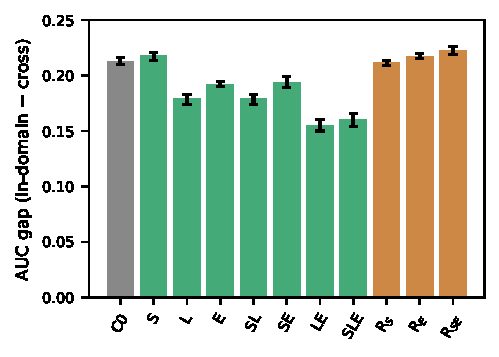
\includegraphics[width=0.78\columnwidth]{fig_gap.pdf}
\caption{Archived protocol: Pooled AUC gap by condition for TF-IDF + LR (mean, 95\% interval over eight seeds). Gray: baseline; green: factorial cells; orange: random-deletion controls. S: source-marker masking, L: length matching, E: entity masking; $R_x$: random deletion matched to $x$.}
\label{fig:gap}
\end{figure}

\begin{table}[t]
\caption{Archived protocol: TF-IDF factorial effects (coded $\pm1$) on cross-dataset AUC and on the AUC gap, 95\% intervals over eight seeds.}
\label{tab:effects}
\centering\footnotesize
\adjustbox{max width=\linewidth}{\begin{tabular}{@{}lcc@{}}
\toprule
Term & Cross AUC & AUC gap\\
\midrule
S & $-0.010$ \ci{-.012}{-.008} & $+0.003$ \ci{-.000}{.006}\\
L & $+0.037$ \ci{.036}{.039} & $-0.036$ \ci{-.038}{-.034}\\
E & $+0.016$ \ci{.012}{.020} & $-0.022$ \ci{-.026}{-.018}\\
S$\times$L & $+0.001$ \ci{-.002}{.004} & $-0.000$ \ci{-.003}{.003}\\
S$\times$E & $-0.000$ \ci{-.002}{.002} & $+0.001$ \ci{-.001}{.002}\\
L$\times$E & $+0.001$ \ci{-.002}{.003} & $+0.001$ \ci{-.002}{.003}\\
S$\times$L$\times$E & $-0.002$ \ci{-.005}{.000} & $+0.002$ \ci{-.000}{.005}\\
\bottomrule
\end{tabular}}
\end{table}

\subsection{Effects differ by dataset pair}
\begin{table}[t]
\caption{Archived protocol: TF-IDF + LR: change in cross-dataset AUC relative to the baseline, per ordered pair (mean over eight seeds; \textbf{bold}: 95\% interval over seeds excludes zero). The first column is the baseline AUC.}
\label{tab:pairs}
\centering\footnotesize
\adjustbox{max width=\linewidth}{\begin{tabular}{@{}lccccccc@{}}
\toprule
Pair (train$\rightarrow$test) & C0 AUC & S & L & E & L+E & S+L+E & $R_E$\\
\midrule
ISOT$\rightarrow$McIntire & .622 & $-.014$ & \textbf{+.055} & \textbf{+.015} & \textbf{+.072} & \textbf{+.065} & +.002\\\\
ISOT$\rightarrow$residual & .632 & $-.003$ & \textbf{+.036} & $-.003$ & \textbf{+.039} & \textbf{+.040} & $-.004$\\\\
McIntire$\rightarrow$ISOT & .738 & $\mathbf{-.040}$ & \textbf{+.069} & \textbf{+.055} & \textbf{+.141} & \textbf{+.115} & $\mathbf{-.017}$\\\\
McIntire$\rightarrow$residual & .915 & $-.009$ & $\mathbf{-.012}$ & $-.007$ & $\mathbf{-.019}$ & $\mathbf{-.023}$ & $-.002$\\\\
residual$\rightarrow$ISOT & .804 & $-.005$ & \textbf{+.075} & \textbf{+.022} & \textbf{+.098} & \textbf{+.083} & $-.013$\\\\
residual$\rightarrow$McIntire & .923 & $-.006$ & $\mathbf{-.020}$ & $-.002$ & $\mathbf{-.015}$ & $\mathbf{-.033}$ & $-.007$\\\\
\bottomrule
\end{tabular}}
\end{table}

Table~\ref{tab:pairs} and Fig.~\ref{fig:heat} show that the pooled picture hides large differences between pairs. Length matching and entity masking raise cross-dataset AUC for all four transfers involving ISOT (L+E: $+0.039$ to $+0.141$). For the two transfers between McIntire and the residual, which already start from high AUC (0.915--0.923), length matching and L+E \emph{lower} AUC slightly (L: $-0.012$ and $-0.020$; L+E: $-0.019$ and $-0.015$; all four intervals exclude zero). This matches the direction of the length confound: in ISOT the fake articles are longer (448 vs.\ 395 words on average), whereas in McIntire and the residual the real ones are (939 vs.\ 709; 895 vs.\ 640). A length cue learned on ISOT misleads on the other two datasets, whereas a cue learned on McIntire transfers to the residual because they share its direction. The pooled gain is therefore driven by ISOT-involving pairs. ISOT-trained models remain weak even after masking (cross AUC 0.67--0.69 for S+L+E), so most of the unexplained gap lies in transfers from ISOT.

\begin{figure}[t]
\centering
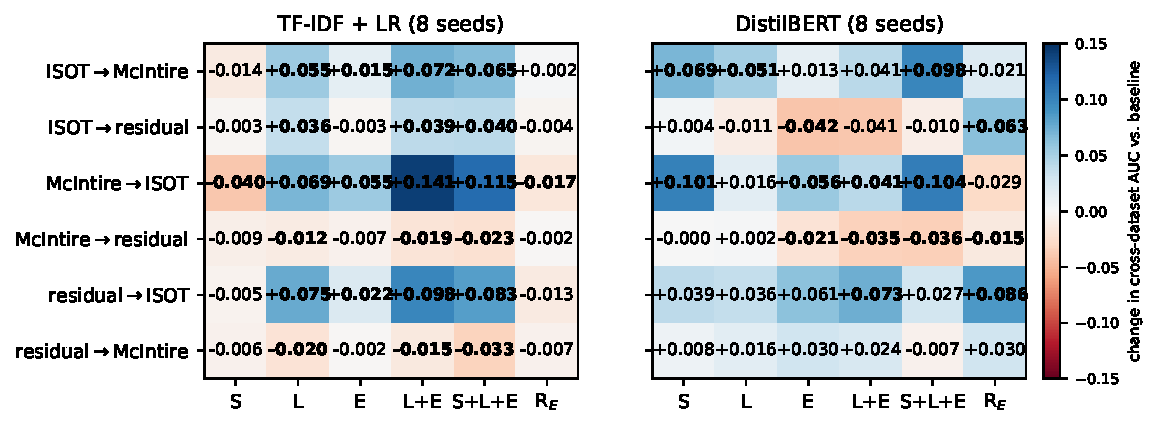
\includegraphics[width=0.92\textwidth]{fig_heatmap.pdf}
\caption{Archived protocol: Change in cross-dataset AUC relative to the baseline for each ordered pair (train $\rightarrow$ test) and intervention (TF-IDF + LR left, DistilBERT right; eight seeds each). S: source-marker masking, L: length matching, E: entity masking, combinations joined by +; $R_E$: random deletion matched to E. Bold: 95\% interval over seeds excludes zero. ``residual'' denotes the WELFake residual, and both panels share one colour scale.}
\label{fig:heat}
\end{figure}

\subsection{Exploratory analyses: source split and temporal expressions}
Table~\ref{tab:expl} reports two post-hoc analyses. Splitting S shows that the harm comes from the web-boilerplate part (share prompts, advertisements, credits, embeds, URLs): its removal changes cross-dataset AUC by $-0.014$ \ci{-0.019}{-0.010} (all eight seeds) and widens the gap by 0.009, whereas removing wire/outlet markers is neutral. A plausible reading is that such boilerplate is shared across low-quality sites and therefore transfers; it is an artifact for content-based judgement but a genuine signal of publisher type. Removing temporal expressions does not help either: it lowers cross-dataset AUC by 0.014 (eight of eight seeds; 0.012 below a size-matched random deletion), and S+L+E+T is 0.013 below S+L+E. We had expected a collection-window artifact to drive McIntire--residual transfer; the data do not support that. Both analyses are exploratory.

\begin{table}[t]
\caption{Archived protocol: Exploratory TF-IDF analyses: change in cross-dataset AUC vs.\ the baseline and vs.\ a random-deletion control of the same size, and change in AUC gap vs.\ baseline (95\% intervals over seeds).}
\label{tab:expl}
\centering\footnotesize
\adjustbox{max width=\linewidth}{\begin{tabular}{@{}lccc@{}}
\toprule
Intervention & $\Delta$AUC vs C0 & $\Delta$AUC vs random & $\Delta$gap vs C0\\
\midrule
S$_W$ (wire/outlet) & $-.000$ \ci{-.004}{.003} & $+.006$ \ci{.003}{.008} & $-.003$ \ci{-.006}{.000}\\
S$_B$ (web boilerplate) & $-.014$ \ci{-.019}{-.010} & $-.013$ \ci{-.019}{-.007} & $+.009$ \ci{.005}{.013}\\
T (temporal) & $-.014$ \ci{-.018}{-.009} & $-.012$ \ci{-.019}{-.004} & $+.011$ \ci{.005}{.016}\\
\bottomrule
\end{tabular}}
\end{table}

\subsection{Robustness to residual duplicates}
\label{sec:robust}
We flagged 207 of 61,197 documents in the analysis set that were exact, prefix or near-duplicates of a document in another dataset, or that were near-empty after stripping source markers (ISOT 63, residual 144; McIntire none, by construction). Of these, 94 of 22,005 fell in the sampling universe (0.43\%). We reran the baseline, the key interventions and the random controls without them, on all eight seeds, for both models, and compared each pooled and pair-level estimate with the main run.

\emph{TF-IDF} (baseline, L, E, L+E, $R_E$, $R_{SE}$). The pooled baseline cross-dataset AUC went from 0.772 to 0.773, and the effects of L ($+0.034$ in both runs), E ($+0.013$ to $+0.014$), L+E ($+0.053$ to $+0.054$) and E against its random control ($+0.020$ in both runs) changed by at most 0.001 \ci{-0.003}{0.006}; the AUC gaps changed by at most 0.002. None of the 24 pair-level effects changed sign, the largest absolute change was 0.012 (length matching, residual$\rightarrow$ISOT), and the median was 0.003. These changes are smaller than the seed-to-seed standard deviation of the effects themselves (0.003--0.007).

\emph{DistilBERT} (baseline, L, E, L+E, S+L+E). The pooled baseline went from 0.805 to 0.806, and the pooled effects changed by at most 0.004 (L: $+0.018$ to $+0.014$; E: $+0.016$ to $+0.015$; L+E: $+0.017$ to $+0.019$; S+L+E: $+0.029$ to $+0.026$), with all intervals for the change spanning roughly $\pm0.02$ to $\pm0.04$; the AUC gaps changed by at most 0.004. Three of the 24 pair-level effects changed sign: length matching on ISOT$\rightarrow$residual ($-0.011$ to $+0.024$) and on residual$\rightarrow$ISOT ($+0.036$ to $-0.026$), and S+L+E on ISOT$\rightarrow$residual ($-0.010$ to $+0.001$). All three involve cells whose original effect was close to zero or whose seed-to-seed interval is wide; the largest absolute change was 0.062 and the median 0.006. These changes are within DistilBERT's run-to-run variation (standard deviation of the pooled effects 0.021--0.030), so the check cannot rule out small contamination effects for DistilBERT, though the changes do not alter any of the primary conclusions reported in this paper. The cleaned runs draw slightly different samples, so the differences include sampling noise as well as any effect of the removed documents.

\subsection{DistilBERT: random deletion as a non-specific perturbation}
\label{sec:bert}
DistilBERT has a higher baseline cross-dataset AUC than TF-IDF (0.805 vs.\ 0.772) and a smaller gap (0.192 vs.\ 0.213). Source masking, S+E and S+L+E raise its cross-dataset AUC by 0.029 to 0.037 over the baseline (S: 0.805 to 0.842), and S+L+E removes 16.7\% of the gap \ci{9.6}{23.8}. But deleting the same number of random words gives almost the same gain (Fig.~\ref{fig:bertctl}): $R_S$, $R_E$ and $R_{SE}$ give 0.831, 0.832 and 0.825, and random deletion alone removes 11--14\% of the gap. The specific effects of targeted removal are not distinguishable from zero: S $-$ $R_S$ is $+0.011$ \ci{-0.009}{0.030}, E $-$ $R_E$ is $-0.010$ \ci{-0.025}{0.005}, and S+E $-$ $R_{SE}$ is $+0.009$ \ci{-0.002}{0.020}. These results are consistent with random token deletion acting as a general, regularization-like perturbation for DistilBERT under this protocol (random word dropping is also used as a training-time augmentation~\cite{zhu2022endef}), an effect TF-IDF does not show, and without the random controls one would conclude that source masking improves generalization by 0.037 AUC. Length matching and entity masking have no clear pooled effect (L: $+0.018$ \ci{-0.006}{0.043}; E: $+0.016$ \ci{-0.004}{0.037}); DistilBERT reads only the first 256 tokens, so document length is largely invisible to it. At pair level (Fig.~\ref{fig:heat}), S+L+E raises transfer for ISOT$\rightarrow$McIntire ($+0.098$ \ci{0.081}{0.115}) and McIntire$\rightarrow$ISOT ($+0.104$ \ci{0.074}{0.134}) and lowers it for McIntire$\rightarrow$residual ($-0.036$ \ci{-0.044}{-0.027}), the same signs as for TF-IDF; the other three pairs are inconclusive, and the matched pair-level control for S+L+E is reported in Section~\ref{sec:matched}. Run-to-run variation is large: with three seeds the S+L+E estimate for residual$\rightarrow$McIntire was $-0.047$ with an interval excluding zero, whereas with eight it is $-0.007$ \ci{-0.062}{0.048}.

\emph{Model comparison.} Whether the two models respond differently is judged from the paired seed-wise differences $D_s$ (Table~\ref{tab:models}), not from which model has a significant effect. The specific effects of targeted removal differ between the models: entity masking beats random deletion for TF-IDF ($+0.020$) but not for DistilBERT ($-0.010$ \ci{-0.025}{0.005}), a difference of $D=+0.030$ \ci{0.014}{0.046} that holds in all eight seeds, and source masking is worse than random deletion for TF-IDF ($-0.014$) but not for DistilBERT ($+0.011$ \ci{-0.009}{0.030}), $D=-0.025$ \ci{-0.043}{-0.006}, again in all eight seeds. Because neither DistilBERT effect is individually distinguishable from zero, the supported statement is that the models respond differently, not that DistilBERT responds in the opposite direction. The apparent difference for source masking against the baseline ($D=-0.050$ \ci{-0.070}{-0.029}) largely reflects random deletion helping DistilBERT. For L+E the TF-IDF gain is larger ($D=+0.035$ \ci{0.012}{0.059}, 7 of 8 seeds), and for S+L+E the difference is not established ($+0.012$ \ci{-0.006}{0.030}). Per pair, the entity-specific difference is concentrated in transfers between ISOT and the residual (ISOT$\rightarrow$residual $+0.105$ \ci{0.064}{0.147}; residual$\rightarrow$ISOT $+0.060$ \ci{0.036}{0.084}; both 8 of 8 seeds). With 30 per-pair contrasts and no correction, per-pair differences are exploratory.

\begin{table}[t]
\caption{Archived protocol: Model comparison, cross-dataset AUC: pooled effect of each contrast for each model and the paired seed-wise difference $D=$ TF-IDF $-$ DistilBERT (mean and 95\% interval over eight seeds).}
\label{tab:models}
\centering\scriptsize\setlength{\tabcolsep}{2pt}
\resizebox{\columnwidth}{!}{%
\adjustbox{max width=\linewidth}{\begin{tabular}{@{}lccc@{}}
\toprule
Contrast & TF-IDF & DistilBERT & $D$\\
\midrule
L $-$ C0 & $+.034$ \ci{.028}{.039} & $+.018$ \ci{-.006}{.043} & $+.015$ \ci{-.007}{.038}\\
L+E $-$ C0 & $+.053$ \ci{.048}{.058} & $+.017$ \ci{-.008}{.042} & $+.035$ \ci{.012}{.059}\\
S+L+E $-$ C0 & $+.041$ \ci{.037}{.046} & $+.029$ \ci{.012}{.047} & $+.012$ \ci{-.006}{.030}\\
S $-$ C0 & $-.013$ \ci{-.019}{-.007} & $+.037$ \ci{.013}{.060} & $-.050$ \ci{-.070}{-.029}\\
S $-$ $R_S$ & $-.014$ \ci{-.019}{-.009} & $+.011$ \ci{-.009}{.030} & $-.025$ \ci{-.043}{-.006}\\
E $-$ $R_E$ & $+.020$ \ci{.016}{.024} & $-.010$ \ci{-.025}{.005} & $+.030$ \ci{.014}{.046}\\
S+E $-$ $R_{SE}$ & $+.016$ \ci{.010}{.022} & $+.009$ \ci{-.002}{.020} & $+.007$ \ci{-.002}{.017}\\
\bottomrule
\end{tabular}}}
\end{table}

\begin{figure}[t]
\centering
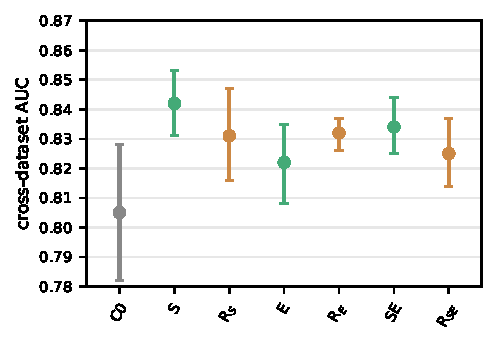
\includegraphics[width=0.78\columnwidth]{fig_bert_controls.pdf}
\caption{Archived protocol: DistilBERT cross-dataset AUC (mean, 95\% interval over eight seeds): baseline (gray), real masking (green) and size-matched random deletion (orange). Real masking is not distinguishable from random deletion; the vertical axis starts at 0.78.}
\label{fig:bertctl}
\end{figure}

\subsection{Matched controls under length matching, and a second transformer}\label{sec:matched}
Two gaps remained after the analyses above: S+L+E had no matched random control, and the transformer result rested on a single model. We closed both. Two conditions were added, L+R$_E$ and L+R$_{SE}$, which apply length matching and then delete as many random words as entity masking (respectively source-plus-entity masking) removes; they are the matched controls of L+E and S+L+E. RoBERTa-base was trained with the DistilBERT recipe (Section~\ref{sec:models}) on the same samples and eight seeds. The new conditions were run for all three models. A seed-0 re-run of conditions C0 and L with the multi-GPU runner used for the new cells reproduced the archived DistilBERT results exactly (AUC, F1, accuracy and AP, difference 0.0 in all 18 cells), so archived and new cells are directly comparable.

\paragraph{Pooled results.}
Table~\ref{tab:matched_pooled} gives the pooled contrasts. For TF-IDF, entity masking beats its matched random control also after length matching: L+E exceeds L+R$_E$ by 0.020 [0.015, 0.024] in all eight seeds, and S+L+E exceeds L+R$_{SE}$ by 0.010 [0.004, 0.016] (seven of eight seeds). For neither transformer does targeted removal beat matched random deletion. For DistilBERT the differences are $-0.013$ [$-0.024$, $-0.001$] and $-0.008$ [$-0.014$, $-0.001$] (seven of eight seeds each); for RoBERTa they are $-0.004$ and $-0.001$, with intervals that include zero. Random deletion alone moves the models in different directions and by different amounts: it lowers TF-IDF cross-dataset AUC by 0.012 [0.007, 0.017] (R$_{SE}$ against C0, eight of eight seeds), raises DistilBERT by 0.020 [$-$0.001, 0.042], and raises RoBERTa by 0.102 [0.081, 0.122] (eight of eight). For RoBERTa the baseline cross-dataset AUC is 0.813, and masking raises it by 0.069 (S) to 0.092 (S+L+E), but random deletion raises it more (R$_{SE}$ +0.102). Adding random deletion on top of length matching raises RoBERTa by 0.117 [0.088, 0.146] and DistilBERT by 0.019 [0.003, 0.035], and does nothing for TF-IDF ($-0.003$ [$-0.009$, 0.003]).

\begin{table}[t]
\caption{Archived protocol: Matched-control contrasts in cross-dataset AUC, pooled over the six ordered pairs: mean, 95\% interval over eight seeds, and number of seeds agreeing in sign with the mean. Bold: interval excludes zero (before rounding). Above the rule: the six contrasts treated as primary; below: exploratory.}\label{tab:matched_pooled}
\footnotesize
\adjustbox{max width=\linewidth}{\begin{tabular}{@{}lccc@{}}
\toprule
Contrast & TF-IDF & DistilBERT & RoBERTa \\
\midrule
S $-$ R$_S$ & \textbf{$-$0.014 [$-$0.019, $-$0.009] (8/8)} & +0.011 [$-$0.009, +0.030] (5/8) & \textbf{$-$0.029 [$-$0.042, $-$0.015] (7/8)} \\
E $-$ R$_E$ & \textbf{+0.020 [+0.016, +0.024] (8/8)} & $-$0.010 [$-$0.025, +0.005] (5/8) & $-$0.008 [$-$0.034, +0.018] (5/8) \\
S+E $-$ R$_{SE}$ & \textbf{+0.016 [+0.010, +0.022] (8/8)} & +0.009 [$-$0.002, +0.020] (6/8) & $-$0.008 [$-$0.018, +0.003] (6/8) \\
L $-$ C0 & \textbf{+0.034 [+0.028, +0.039] (8/8)} & +0.018 [$-$0.006, +0.043] (6/8) & $-$0.024 [$-$0.057, +0.009] (6/8) \\
\midrule
L+E $-$ L+R$_E$ & \textbf{+0.020 [+0.015, +0.024] (8/8)} & \textbf{$-$0.013 [$-$0.024, $-$0.001] (7/8)} & $-$0.004 [$-$0.023, +0.016] (5/8) \\
S+L+E $-$ L+R$_{SE}$ & \textbf{+0.010 [+0.004, +0.016] (7/8)} & \textbf{$-$0.008 [$-$0.014, $-$0.001] (7/8)} & $-$0.001 [$-$0.013, +0.011] (5/8) \\
L+R$_{SE}$ $-$ L & $-$0.003 [$-$0.009, +0.003] (4/8) & \textbf{+0.019 [+0.003, +0.035] (7/8)} & \textbf{+0.117 [+0.088, +0.146] (8/8)} \\
R$_{SE}$ $-$ C0 & \textbf{$-$0.012 [$-$0.017, $-$0.007] (8/8)} & +0.020 [$-$0.001, +0.042] (6/8) & \textbf{+0.102 [+0.081, +0.122] (8/8)} \\
\bottomrule
\end{tabular}
}
\end{table}

\paragraph{Model differences.}
Table~\ref{tab:model_diff} compares the models directly through paired seed-wise differences, as in Section~\ref{sec:stats}. The entity-specific advantage of TF-IDF over DistilBERT holds with length matching (L+E against L+R$_E$: $D=+0.032$ [0.019, 0.045], eight of eight seeds), extending the earlier result without length matching ($+0.030$). The two transformers do not differ clearly on the targeted-removal contrasts (all intervals of DistilBERT $-$ RoBERTa include zero except S against R$_S$ and the random-deletion contrasts): source masking is worse than random deletion for RoBERTa but not for DistilBERT ($D=+0.039$ [0.017, 0.062], eight of eight). The effect of random deletion itself differs strongly between transformers, with RoBERTa gaining about 0.08 AUC more than DistilBERT from R$_{SE}$ (DistilBERT $-$ RoBERTa $-0.081$ [$-0.113$, $-0.050$], eight of eight seeds).

\begin{table}[t]
\caption{Archived protocol: Paired seed-wise differences in the pooled contrast between two models (mean, 95\% interval over eight seeds, seeds agreeing in sign). Bold: interval excludes zero.}\label{tab:model_diff}
\footnotesize
\adjustbox{max width=\linewidth}{\begin{tabular}{@{}lccc@{}}
\toprule
Contrast & TF-IDF $-$ DistilBERT & TF-IDF $-$ RoBERTa & DistilBERT $-$ RoBERTa \\
\midrule
S $-$ R$_S$ & \textbf{$-$0.025 [$-$0.043, $-$0.006] (8/8)} & \textbf{+0.015 [+0.000, +0.029] (7/8)} & \textbf{+0.039 [+0.017, +0.062] (8/8)} \\
E $-$ R$_E$ & \textbf{+0.030 [+0.014, +0.046] (8/8)} & \textbf{+0.028 [+0.000, +0.056] (7/8)} & $-$0.002 [$-$0.020, +0.016] (4/8) \\
S+E $-$ R$_{SE}$ & +0.007 [$-$0.002, +0.017] (5/8) & \textbf{+0.024 [+0.010, +0.038] (7/8)} & +0.016 [$-$0.001, +0.034] (6/8) \\
L $-$ C0 & +0.015 [$-$0.007, +0.038] (6/8) & \textbf{+0.058 [+0.024, +0.091] (7/8)} & +0.042 [$-$0.002, +0.087] (6/8) \\
\midrule
L+E $-$ L+R$_E$ & \textbf{+0.032 [+0.019, +0.045] (8/8)} & \textbf{+0.023 [+0.004, +0.042] (6/8)} & $-$0.009 [$-$0.036, +0.018] (4/8) \\
S+L+E $-$ L+R$_{SE}$ & \textbf{+0.018 [+0.007, +0.029] (7/8)} & \textbf{+0.011 [+0.002, +0.021] (7/8)} & $-$0.007 [$-$0.022, +0.009] (6/8) \\
L+R$_{SE}$ $-$ L & \textbf{$-$0.022 [$-$0.039, $-$0.005] (7/8)} & \textbf{$-$0.120 [$-$0.147, $-$0.093] (8/8)} & \textbf{$-$0.098 [$-$0.130, $-$0.067] (8/8)} \\
R$_{SE}$ $-$ C0 & \textbf{$-$0.032 [$-$0.050, $-$0.014] (7/8)} & \textbf{$-$0.113 [$-$0.133, $-$0.093] (8/8)} & \textbf{$-$0.081 [$-$0.113, $-$0.050] (8/8)} \\
\bottomrule
\end{tabular}
}
\end{table}

\paragraph{Dataset pairs.}
The pooled values for S+L+E hide effects of opposite sign (Table~\ref{tab:matched_pairs}, Fig.~\ref{fig:matched_pairs}). For both transformers, S+L+E beats its matched random control on the two transfers between ISOT and McIntire (DistilBERT +0.046 and +0.083, RoBERTa +0.042 and +0.028) and falls below it on transfers involving the WELFake residual (DistilBERT $-0.021$ to $-0.063$, eight of eight seeds for all four; RoBERTa $-0.015$ to $-0.022$, with three of four intervals excluding zero and ISOT$\rightarrow$residual inconclusive). TF-IDF shows no such split: only McIntire$\rightarrow$ISOT is clearly positive ($+0.049$ [0.035, 0.064]), and the other five pairs are inconclusive. For the entity-only contrast (L+E against L+R$_E$) the DistilBERT negatives on transfers into the residual do not appear for RoBERTa, so only the S+L+E pattern replicates across the two transformers. These pair-level contrasts are exploratory: they are 12 uncorrected contrasts per model, and with eight seeds the smallest attainable exact sign-flip $p$ (0.0078) already exceeds the Holm threshold $0.05/12$. We do not explain the pattern; the data do not separate the contribution of source and entity masking per pair.

\begin{table}[t]
\caption{Archived protocol: Per-pair matched-control contrasts in cross-dataset AUC (mean, 95\% interval over eight seeds, seeds agreeing in sign). Bold: interval excludes zero. Exploratory, uncorrected.}\label{tab:matched_pairs}
\footnotesize
\adjustbox{max width=\linewidth}{\begin{tabular}{@{}lccc@{}}
\toprule
Transfer & TF-IDF & DistilBERT & RoBERTa \\
\midrule
\multicolumn{4}{@{}l}{\textit{S+L+E $-$ L+R$_{SE}$}} \\
ISOT$\rightarrow$McIntire & +0.008 [$-$0.008, +0.025] (6/8) & \textbf{+0.046 [+0.023, +0.069] (8/8)} & \textbf{+0.042 [+0.024, +0.061] (8/8)} \\
ISOT$\rightarrow$residual & +0.002 [$-$0.013, +0.017] (5/8) & \textbf{$-$0.063 [$-$0.082, $-$0.043] (8/8)} & $-$0.022 [$-$0.069, +0.025] (6/8) \\
McIntire$\rightarrow$ISOT & \textbf{+0.049 [+0.035, +0.064] (8/8)} & \textbf{+0.083 [+0.057, +0.109] (8/8)} & \textbf{+0.028 [+0.007, +0.048] (7/8)} \\
McIntire$\rightarrow$residual & $-$0.005 [$-$0.012, +0.002] (6/8) & \textbf{$-$0.021 [$-$0.032, $-$0.010] (8/8)} & \textbf{$-$0.022 [$-$0.033, $-$0.010] (7/8)} \\
residual$\rightarrow$ISOT & +0.014 [$-$0.009, +0.037] (6/8) & \textbf{$-$0.062 [$-$0.089, $-$0.035] (8/8)} & \textbf{$-$0.019 [$-$0.031, $-$0.008] (8/8)} \\
residual$\rightarrow$McIntire & $-$0.007 [$-$0.018, +0.003] (7/8) & \textbf{$-$0.030 [$-$0.043, $-$0.017] (8/8)} & \textbf{$-$0.015 [$-$0.025, $-$0.004] (8/8)} \\
\midrule
\multicolumn{4}{@{}l}{\textit{L+E $-$ L+R$_{E}$}} \\
ISOT$\rightarrow$McIntire & \textbf{+0.014 [+0.001, +0.027] (6/8)} & $-$0.008 [$-$0.045, +0.029] (5/8) & $-$0.039 [$-$0.088, +0.011] (6/8) \\
ISOT$\rightarrow$residual & $-$0.003 [$-$0.017, +0.010] (4/8) & \textbf{$-$0.079 [$-$0.127, $-$0.030] (8/8)} & +0.043 [$-$0.020, +0.105] (7/8) \\
McIntire$\rightarrow$ISOT & \textbf{+0.072 [+0.061, +0.083] (8/8)} & +0.038 [$-$0.000, +0.077] (7/8) & $-$0.017 [$-$0.048, +0.013] (6/8) \\
McIntire$\rightarrow$residual & +0.000 [$-$0.007, +0.007] (5/8) & \textbf{$-$0.016 [$-$0.024, $-$0.008] (8/8)} & +0.003 [$-$0.016, +0.023] (3/8) \\
residual$\rightarrow$ISOT & \textbf{+0.029 [+0.013, +0.044] (8/8)} & $-$0.012 [$-$0.052, +0.028] (3/8) & $-$0.008 [$-$0.034, +0.017] (5/8) \\
residual$\rightarrow$McIntire & +0.007 [$-$0.001, +0.014] (6/8) & +0.002 [$-$0.018, +0.021] (5/8) & $-$0.003 [$-$0.013, +0.008] (3/8) \\
\bottomrule
\end{tabular}
}
\end{table}

\begin{figure}[t]
\centering
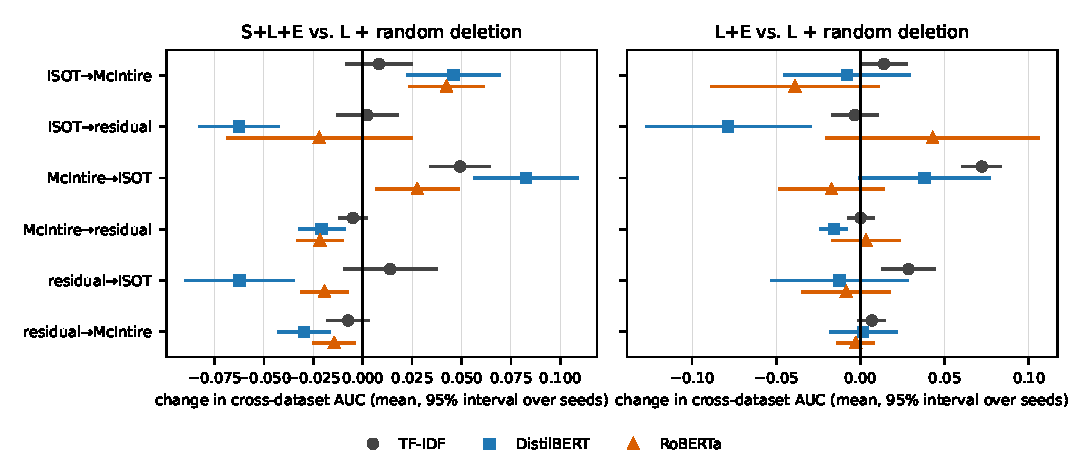
\includegraphics[width=\linewidth]{fig_matched_pairs.pdf}
\caption{Archived protocol: Per-pair matched-control contrasts in cross-dataset AUC for the three models (mean and 95\% interval over eight seeds). Left: S+L+E minus length matching plus random deletion of the same size; right: L+E minus length matching plus random deletion. Points to the right of zero mean targeted removal transfers better than random deletion.}\label{fig:matched_pairs}
\end{figure}

\paragraph{Multiplicity.}
Over the six primary contrasts, the exact paired sign-flip $p$-values of TF-IDF are 0.0078 (five contrasts) and 0.0156 (S+L+E against L+R$_{SE}$), giving Holm-adjusted $p=0.047$ for all six; none of the six contrasts survives Holm correction for DistilBERT or RoBERTa (smallest adjusted $p=0.094$ for both). This family was defined after the earlier exploratory results had been seen, and the sign-flip $p$-values describe stability under resampling within one fixed document universe, so we treat the adjusted values as descriptive and not as confirmatory evidence.
